\documentclass{article}
\usepackage[utf8]{inputenc}
\usepackage{xcolor}
\usepackage{url}
\usepackage[nottoc]{tocbibind}
\usepackage{graphicx}
\usepackage[bottom]{footmisc}
\usepackage{float}

\title{CSCE 479/879 Homework 3: Generative models}
\author{Shubham Bry \\
Shiva Paudel \\
Puranjit Singh \\
Kantilata Thapa} 
%\date{February 2022}

\begin{document}

\maketitle

\begin{abstract} 

Genrative modeling is an unsupervised learning task that involves automatically discovering and learning the regularities or patterns in input data in such a way that model can be used to genrate new examples that possibily could have been drawn from the original dataset. Generative models are powerful techniques that aim at learning the true data distributions from the training data to generate new data points with same variations. The main objective of this homework was to develop a generative model like Generative Adversarial Network (GAN) using CIFAR10 dataset. The main motivation was to develop a GAN on the CIFAR10 dataset and to evaluate its performance. The validation accuracy for the reconstructed images was calculated to be ... during the training phase. The FID score for the new instances generated was around 1.78.

\end{abstract}

\section{Introduction}
\label{sec:intro}

The main goal for this homework assignment 3 was to develop a generative model like a variational autoencoder (VAE) or a generative adversarial network (GAN) either using CelebA dataset or a dataset like CIFAR10. We chose CIFAR10 dataset to work on this problem because the training process was quite easier and faster in CIFAR10 dataset than that of CelebA dataset. Working with a familiarized dataset such as CIFAR10 helps us focus more on aspects such as architectural tuning and variations in the sets of hyper-parameters used in our homework. Also, this helped us to train the model in a lesser amount of time for the image generation process. 

Specifically, we used a generative adversarial network (GAN) for this homework assignment. The GAN (Generative Adversarial Network) consists of two models, the generator model, and the discriminative model. A generator network takes a sample from random noise and generates sample of data and discriminator network decides whether the data is generated or taken from the real sample using a binary classification problem with the help of sigmoid function that gives the output in a range between 0 and 1. Generative model analyzes the distribution of the data in such a way that after the training phase the probability of discriminator making a mistake maximizes and the discriminator on the other hand is based on a model that will estimate the probability that the sample is coming from the real data or the generator.  

We used discriminator model which has 4 convolution layers with stride size of $2\times2$ to down sample the input image. For the generator architecture, it requires to transform a vector from the latent space with 100 dimensions to a 2D array with $32\times32\times3$ or 3,072 values. 48 nodes were used to represent a low resolution output image in the inital layer. The crucial operation for this architecture was up sampling of low resolution images which was achieved by sampling with Conv2D Transpose layer. The stride of size $2\times2$ was used after every Conv2D transpose layer. Similarly, kernel size of $4\times4$ was used to avoid a checkerboard pattern. Finally, the FID score of 1.78 was obtained to evaluate the model performance \cite{Jason}. 


\section{Problem Description}
The major problem of this homework assignment is to build a generative model based on VAE (Variational Auto Encoder) or GANs (Generative Adversarial Network) to train and generate new samples from the CelebA image datasets or other datasets. We used CIFAR10 datasets and GAN model to address the specific problem for this homework assignment.  

\subsection{CIFAR10 datasets}
CIFAR10 dataset consists of 60,000, $32\times32$-pixel color images of objects with 10 classes, 6000 images per class. The 10 classes present in the dataset are airplane, automobile, bird, cat, deer, dog, frog, horse, ship, and truck \cite{kaggle}. These are exceedingly small images, much smaller than a typical photograph. Therefore, they can be developed and trained quickly, allowing focus to be put on the model architecture and image generation process itself.  

\subsection{Approaches}
Generative Adversarial Network (GAN) is an approach for fitting convolution neural networks to generate images. 
Building a GAN to generate images requires two different models, one discriminator convolutional neural network model to classify whether a given image is real or another generator model to generate a fake image. 

\begin{figure}[H]
    \centering
    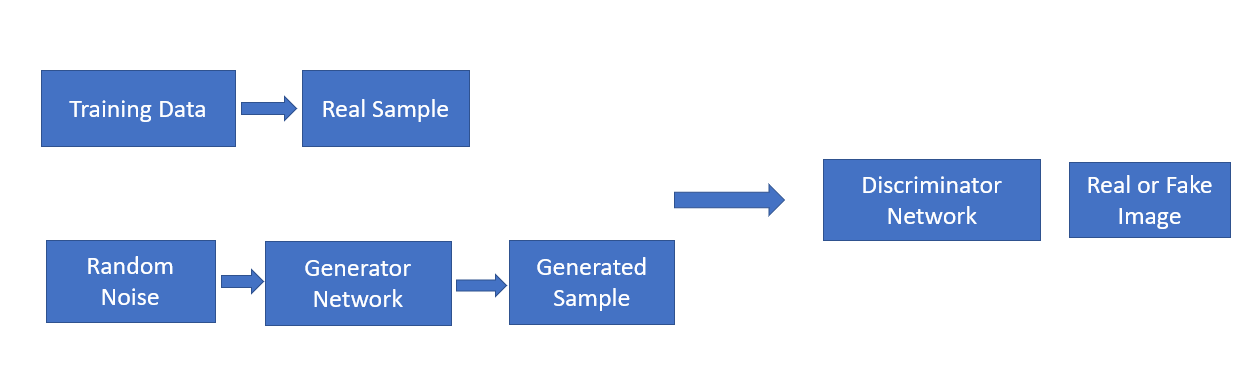
\includegraphics[width=\textwidth]{Generator workflow.PNG}
    \caption{ Workflow of GANs(Generative Adversarial Network}
    \label{fig:compute}
\end{figure}



To generate an image generator model uses an inverse convolution layer to transform an input to a full two-dimensional image of pixel values. We defined a discriminator model, which takes an image with three color channels and $32\times32$ pixels as input and classifies the image whether it is real or fake(generated). Our discriminator model has four convolution layers with stride size of $2\times2$ to down sample the input image. For this model we used ‘Adam’ as optimizer. The architecture of fig \ref{fig:compute1} is our discriminator model.  

\begin{figure}[H]
    \centering
    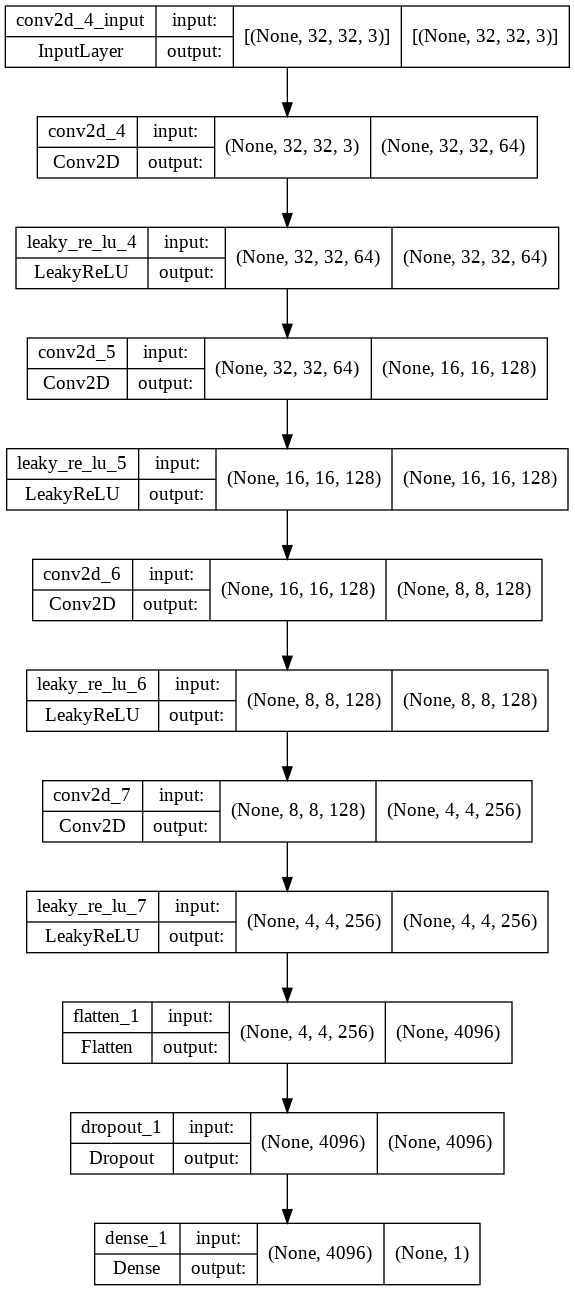
\includegraphics[width=0.5\textwidth]{d_model.png}
    \caption{ Discriminator Model Architecture}
    \label{fig:compute1}
\end{figure}

The generator architecture, fig \ref{fig:compute2} generates the fake image. This model takes latent space an arbitrarily defined vector space of Gussian-distributed values as input and a square color image as output. Developing a generator model requires that we transform a vector from the latent space with 100 dimensions to a 2D array with $32\times32\times3$, or 3,072 values \cite{goodfellow2014generative}. We achieve this by deep convolutional generative adversarial networks. The initial layer in the generator model is a dense layer which has enough nodes to represent a low resolution version of the output image. We used a dense layer with 48 nodes to represent a low resolution output image. The crucial operation here is upsampling of this low resolution image. We achieve this by sampling with the Conv2DTranspose layer. In our architecture we are using stride size of $(2\times2)$ to double after every Conv2DTranspose layer. It is also important to notice that we are using kernel size of $(4\times4)$ to avoid a checkerboard pattern. We repeated this layer unless we get an output image of size $32\times32$. The generator model weights are updated based on the performance of the discriminator model. The updates on the generator model are based on the classification results from the discriminator model, better the discriminator model performs higher will be the generator update. Finally, both the models were put together with a GAN model to fit both the models.  

\begin{figure}[H]
    \centering
    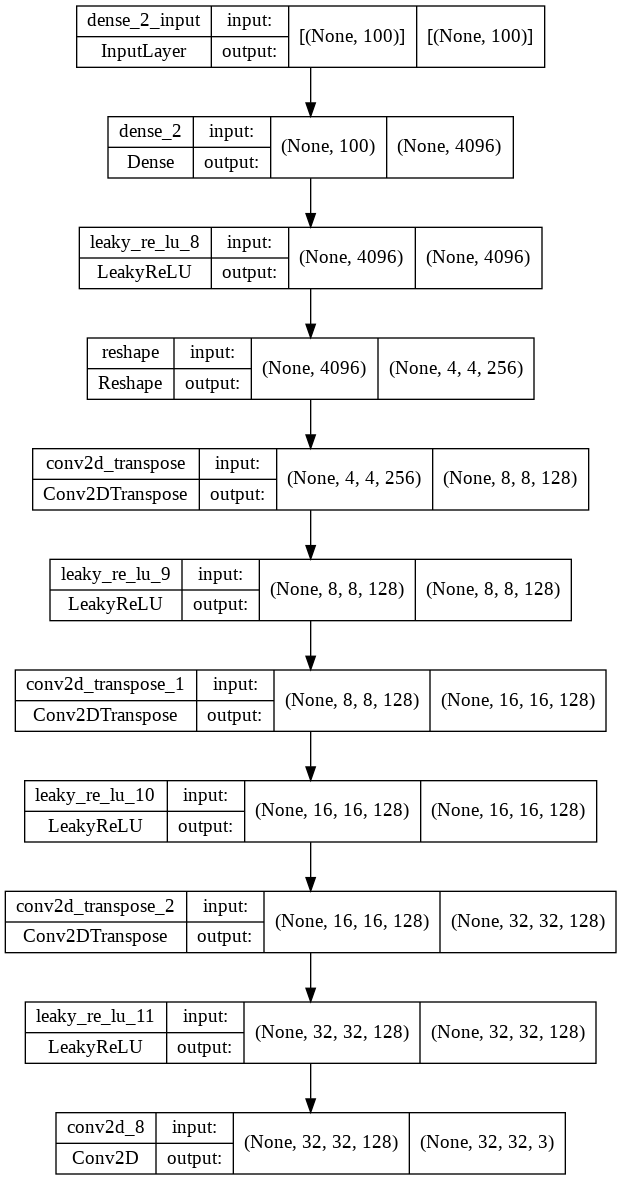
\includegraphics[width=0.5\textwidth]{g_model.png}
    \caption{ Generator Model Architecture}
    \label{fig:compute2}
\end{figure}
  

It was tricky to evaluate the performance of the GAN model as we cannot calculate error scores for generated images. To make the training process easier and effective, we calculated FID ( Fréchet Inception Distance) scores on real and fake images. We programme the model to stop on training after our model performance i.e. FID score is similar for 5 epochs. 



 \iffalse

\section{Approaches}

\subsection{Fashion MNIST dataset}

For the classification of Fashion-MNIST dataset=, two model architectures were developed and parameters such as accuracy were observed on training  and testing datasets. During the pre-processing the pixel value of training images and testing images were divided by 255 to convert them to one-hot vector. A detailed description of each model architecture is given below:

In the first model architecture we used a single fully connected dense layer. Specifically, in this model we analyzed output performance of four hyper-parameters, namely dropout, ReLu activation function, Adam optimizer and learning rate.
\begin{itemize}
    \item \textbf{Trial Run 1:} A single hidden layer of 200 neurons without dropout, no L2 regularization and no learning rate was applied.
    \item \textbf{Trial Run 2:} Dropout of 0.2 and L2 regularization was added with the learning rate of 0.001.
    \item \textbf{Trial Run 3:} Dropout was changed to 0.05 for the same layer and l2 regularization with a learning rate of 0.001 was applied and subsequent results were analyzed.
    \item \textbf{Trial Run 4:} Fourth, everything was left similar, we changed the learning rate to 0.0001 and the result was analyzed to see how slow or fast the model learns.
\end{itemize}

The 2 layout in the follwoing figure \ref{fig:compute} describe the 2 approaches used in Model Architecture 1. The layer on left depicts a layout in which no dropout layer is used in the model (as in Trial Run 1) and in the layout present on the right side depicts use of Dropout in between Dense fully connected layers.

\begin{figure}[H]
    \centering
    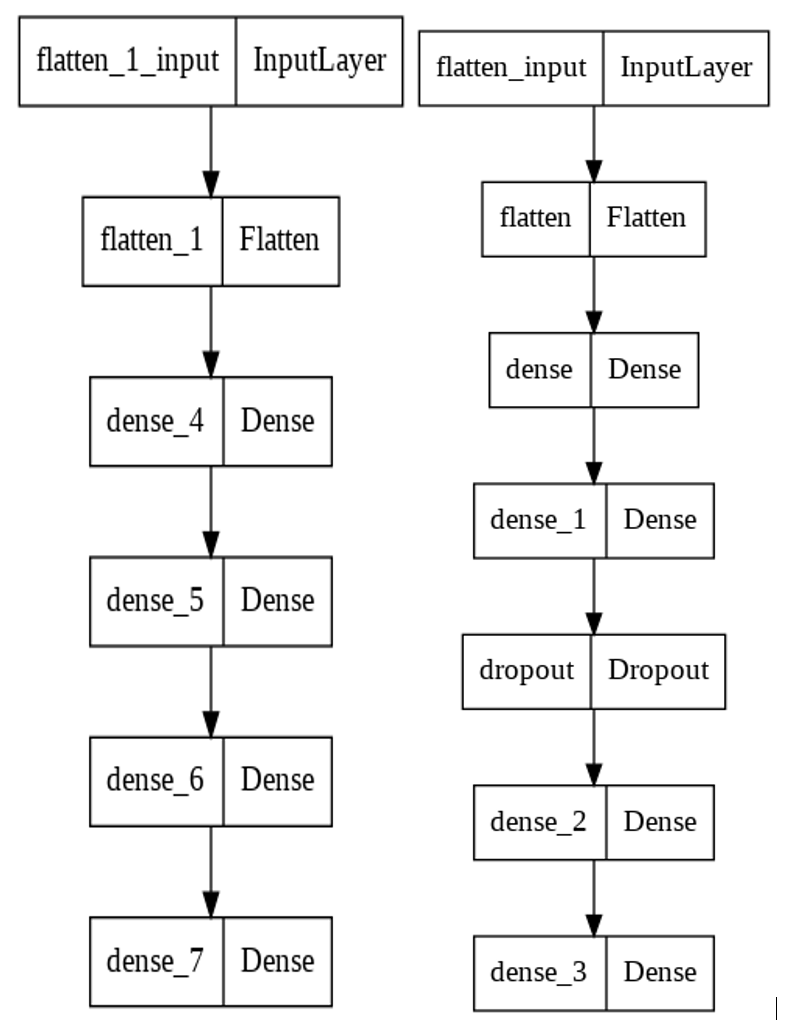
\includegraphics[width=0.5\textwidth]{Capture.PNG}
    \caption{Fashion MNIST Architecture 1 with various trail run}
    \label{fig:compute}
\end{figure}

In the second model architecture following changes were made in the existing model. A few more hidden layers were added and a variation in drop out was made. Use of ReLu activation function, Adam optimizer and variable learning rate was left as it was in architecture 1. Addition of more layers increases the validation accuracy of the model and the drop out layer reduces the over fitting problem like mentioned in the previous architecture. Also, different batch sizes were used for training in this architecture.

\begin{itemize}
    \item \textbf{Trial Run 1:} Four hidden layers in the model were applied with 20\% dropout, 0.0001 learning rate and beta of 0.95 and L2 regularization was applied at every dense layer. 
    \item \textbf{Trial Run 2:} In this trial, dropout was changed to 50\%, learning rate was increased to 0.0005 and L regularization was applied to every dense layer.
    \item \textbf{Trial Run 3 and 4:} In the last two trials we wanted to see what difference batch size makes in performance, so model was trained with two different batch size i.e., 32 and 64 with a learning rate of 20\%.
\end{itemize}

\begin{figure}[H]
    \centering
    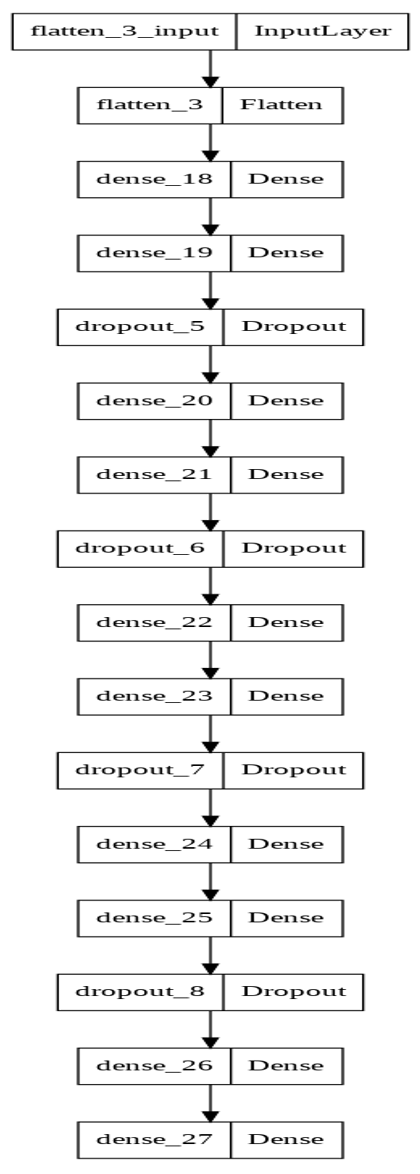
\includegraphics[with=\textwidth, height = 19cm]{Capture1.png}
    \caption{Fashion MNIST architecture 2 with various trail run}
    \label{fig:MNISTAc2}
\end{figure}

\subsection{CIFAR-100 dataset}

For classification of CIFAR-100, we tried three different architectures based on convolution neural networks, to observe changes in model's performance and efficiency.

\begin{itemize}
    \item \textbf{First:} We implement the simplest architecture with two convolution , max-pooling layers continued with a Flatten and two dense layers respectively.
    \item \textbf{Second:} Convolutional architecture were implemented with a residual block.
    \item \textbf{Third:} Deeper Convolutional architecture were implemented with a residual block and a bottleneck in series. 
\end{itemize}

The fig. \ref{fig:Cifar100A1} shows our first architecture. This is the simplest sequential architecture model with two convolution layers, two max-pooling layers and two fully connected layers at the end. In the first convolution we are using 32 filters with kernel size of (3, 3) followed by max-pooling layers. In the following convolutional layer 64 filters of same kernel size were used with pooling layers. Finally, two dense layers with 100 nodes each were added. In this architecture we wanted to see how well the model performs with the simplest possible architecture.

\begin{figure}[H]
    \centering
    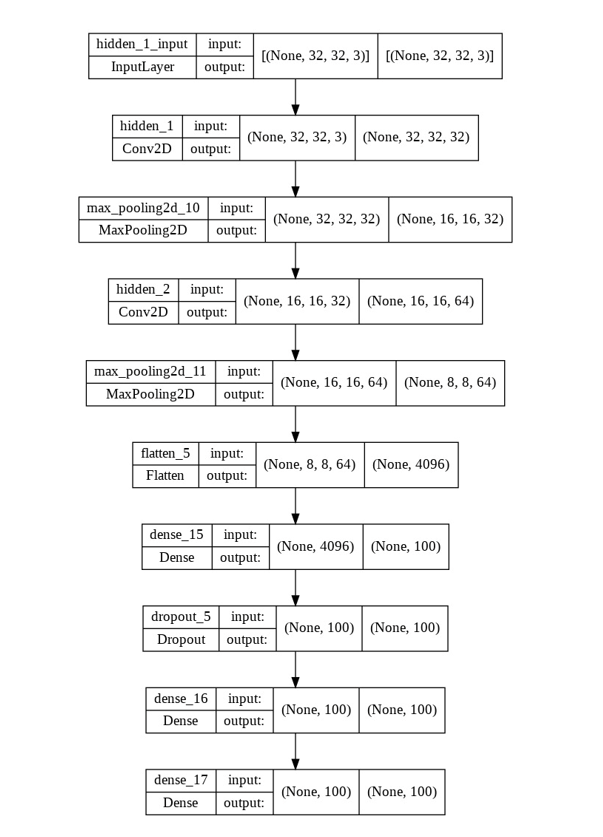
\includegraphics[with=\textwidth]{Capture2.png}
    \caption{CNN Architecture 1 for CIFAR-100}
    \label{fig:Cifar100A1}
\end{figure}

In the second architecture shown in fig. \ref{fig:Cifar100A2} we decided to add more convolution layers in sequential mode. In total, we added 7 more convolution layers and 6 more max-pooling layers to our predefined architecture. With this architecture we were trying to observe whether we can improve the performance by adding more sequential layers. We also added linear regularization l2 and dropout layers for further regularization.

\begin{figure}[H]
    \centering
    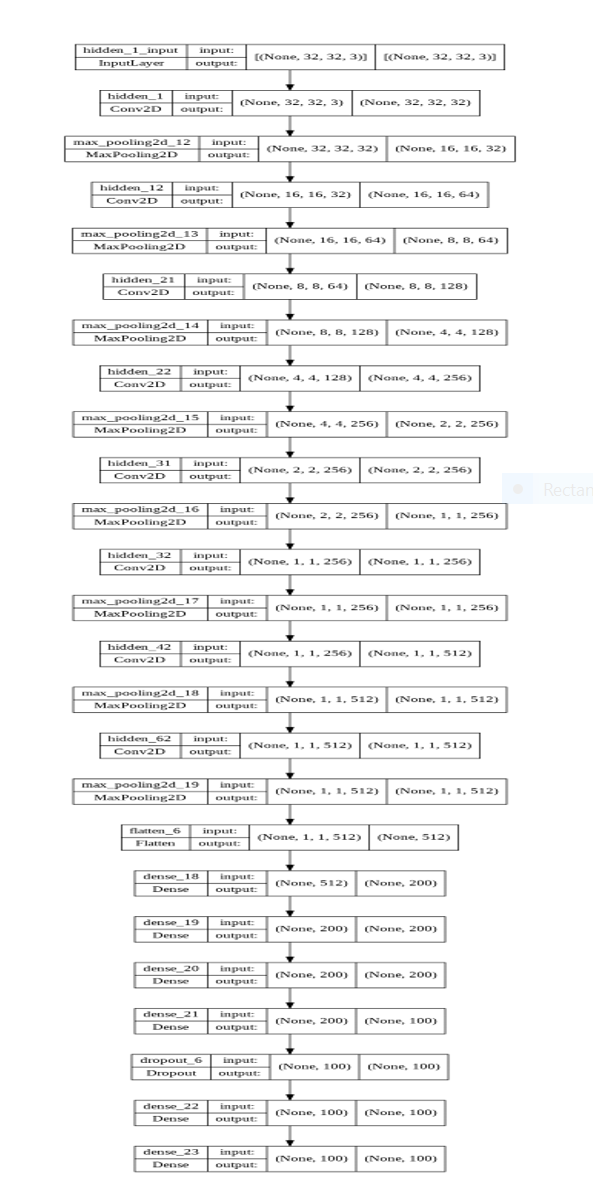
\includegraphics[with=\textwidth, height = 20cm]{Capture3.PNG}
    \caption{CNN Architecture 2 for CIFAR-100}
    \label{fig:Cifar100A2}
\end{figure}

In the final architecture we tried to implement simplest residual architecture as shown in fig. \ref{fig:Cifar100A3}. In this architecture we tried to implement one residual architecture and one bottleneck architecture in series to check how well the model performs in comparison to the previous two models. Figures \ref{fig:ResidualB} and fig. \ref{fig:ResidualBConv} show the flowcharts of residual block, here the skip connection jumps over some layers. Skipping the layers in the initial training stages effectively simplifies the network. This speeds the learning pace by reducing the vanishing gradient problem. In our model we are skipping two convolution layers and two batch normalization layers by each feed-forward. We implemented this architecture to see if our lower validation accuracy is due to the vanishing gradient problem.

\begin{figure}[H]
    \centering
    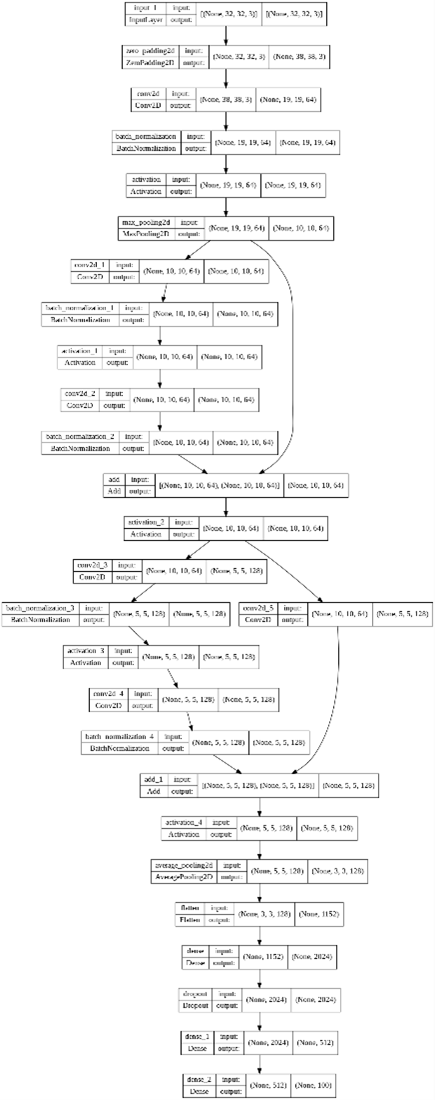
\includegraphics[with=\textwidth, height=20cm]{Picture1.png}
    \caption{CNN Architecture 3 for CIFAR-100}
    \label{fig:Cifar100A3}
\end{figure}

\begin{figure}[H]
    \centering
    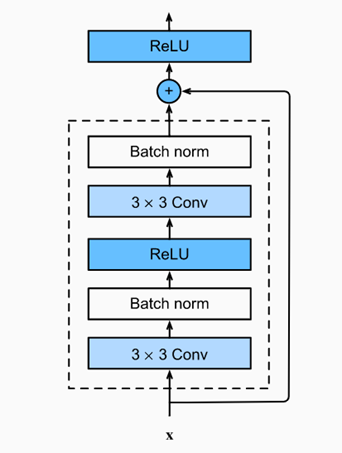
\includegraphics[with=\textwidth, height=8cm]{Picture2.png}
    \caption{Residual Architecture}
    \label{fig:ResidualB}
\end{figure}

\begin{figure}[H]
    \centering
    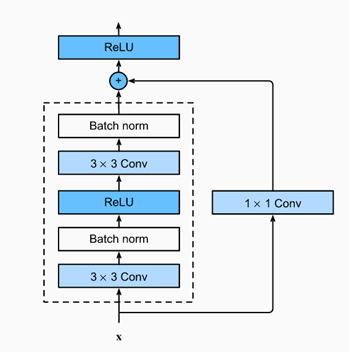
\includegraphics[with=\textwidth, height=8.5cm]{Picture3.png}
    \caption{Residual Architecture with Convolution}
    \label{fig:ResidualBConv}
\end{figure}


The model architecture that achieved the best validation accuracy for CIFAR-100 dataset was the model based on residual architecture. Notable changes in training efficency were observed in comparison between the three architectures but no significant changes in the validation efficiency were observed.
\fi

\section{Experimental Setup}
This section describes the process we used for training the GANs model so that the readers can replicate the implementation if needed. 
\subsection{Data Sources}
To implement and train the GANs, we used CIFAR10 datasets \cite{kaggle}. This dataset was imported from keras API. The dataset was divided into five training batches and one test batch, with 10000 images each. The test batch contains exactly 1000 randomly selected images from each class. The training batches contain the remaining images in random order, but some training batches may contain more images from one class than another. Amongst them, the training batches contain exactly 5000 images from each class.

\subsection{Pre-processing}
For preprocessing of the datasets, keras provides access to the CIFAR10 dataset via cifar10.load\_dataset() function. The pixel values of the images were scales from the range of unsigned integers in [0,255] to the normalized range of [-1,1]. 

\subsection{Performance Measures}
\subsubsection{FID (Fréchet Inception Distance) Score } 

The FID score was used to evaluate the quality of images generated by generative adversarial networks, and lower scores have been shown to correlate well with higher quality images. To maintain consistency in the quality of the images that are generated, FID metrics were used. Lower scores indicate the two groups of images are more similar, or have more similar statistics, with a perfect score being 0.0 indicating that the two groups of images are identical. In other words, the similarity between real and generated images is close. FID compares the statistics of generated samples to real samples, instead of evaluating generated samples in a vacuum \cite{lucic2018gans}. 

\subsubsection{Generator Loss}

While the generator is trained, it samples random noise and produces an output from that noise. The output then goes through the discriminator and gets classified as either “Real” or “Fake” based on the ability of the discriminator to tell one from the other. The generator loss is then calculated from the discriminator’s classification – it gets rewarded if it successfully fools the discriminator and gets penalized otherwise.
\begin{equation}
    \nabla_\theta\frac{1}{m}\sum_{i=1}^{m}log\left( 1-D\left( G(z^{\left( i \right)}) \right) \right)
\end{equation}

The following equation is minimized to training the generator: 

\subsubsection{Discriminator Loss}

While the discriminator is trained, it classifies both the real data and the fake data from the generator. 

It penalizes itself for misclassifying a real instance as fake, or a fake instance (created by the generator) as real, by maximizing the function below. 
\begin{equation}
    \nabla_\theta\frac{1}{m}\sum_{i=1}^{m}\left[ logD\left( x^{\left( i \right)} \right)+\left( 1-D\left( G\left(z ^{i} \right) \right) \right) \right]
\end{equation}


$log(D(x))$ refers to the probability that the generator is rightly classifying the real image, 

maximizing $log(1-D(G(z)))$ would help it to correctly label the fake image that comes from the generator \cite{Jason1}. 

 
\iffalse


\begin{table}[h]
 \caption{Summary of hyperparameters used for Fashion-MNIST}
    \begin{tabular}{|c|c|c|c|c|c|} \hline
      Model   & Hidden Layers & Dropout & L2 Regularization & Learning Rate & Batch size\\
    Arch1 TR1 & 3 & 0 & Not used & 0 & 32\\
    Arch1 TR2 & 3 & 0.2 & Used & 0.001 & 32\\
    Arch1 TR3 & 3 & 0.05 & Used & 0.001 & 32\\ 
    Arch1 TR4 & 3 & 0.05 & Used & 0.0001 & 32\\
    Arch2 TR1 & 9 & 0.2 & Used & 0.0001 & 32\\
    Arch2 TR2 & 9 & 0.5 & Used & 0.0005 & 32\\
    Arch2 TR3 & 9 & 0.2 & Used & 0.0005 & 32\\
    Arch2 TR4 & 9 & 0.2 & Used & 0.0005 & 64\\\hline
    \end{tabular}
 
    \label{tab:CNN-perf}
\end{table}

\noindent Note : 200 neurons were used in each Train Run in the above mentioned architectures.
\fi

\section{Experimental Results}
As mentioned in Section 3, the model architectures were run for 200 epochs with early stopping callbacks and patience factor of 5. We can see from the results of FID values plotted in the following plot show that the values of FID was fluctuating around 2 after training model for 25 epcohs. We know that less is the FID value more is the simlarity between the original and genrated images. Observing values of FID around 2 in the training phase makes sense because we have 50000 images in our training dataset and only 5000 images per each class which is also a limitation in training these GAN better. Training GAN on CelebA dataset generates better results as compared to CIFAR10 dataset because there are approximately 200000 images present in the former.  

\begin{figure}[H]
    \centering
    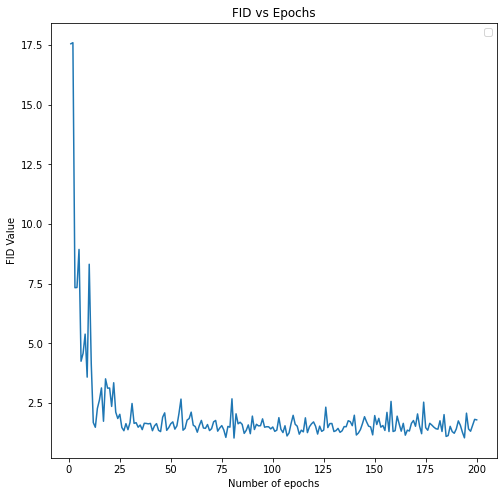
\includegraphics[width=\textwidth]{FID.png}
    \caption{FID values vs No. of Epochs}
    \label{fig:compute}
\end{figure}

\begin{figure}[H]
    \centering
    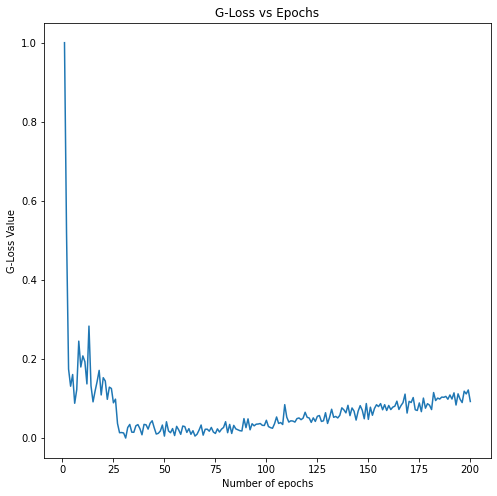
\includegraphics[width=\textwidth]{G_Loss.png}
    \caption{G loss values vs No. of Epochs}
    \label{fig:compute}
\end{figure}

\begin{figure}[H]
    \centering
    \includegraphics[width=\textwidth]{D_Loss.png}
    \caption{D loss values vs No. of Epochs}
    \label{fig:compute}
\end{figure}


\begin{figure}[H]
    \centering
    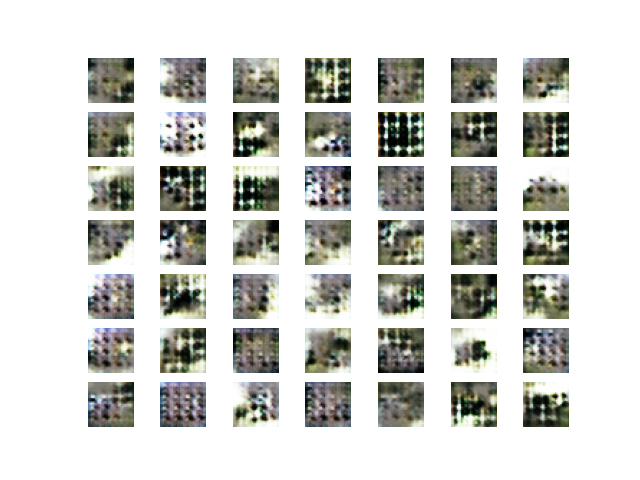
\includegraphics[width=\textwidth]{e10.png}
    \caption{Generated Image on 10 Epochs}
    \label{fig:compute}
\end{figure}
The result from generator model after 10 epochs are very low in quality but still some differences between background and foreground can be seen with a blog in the middle of each image. 


\begin{figure}[H]
    \centering
    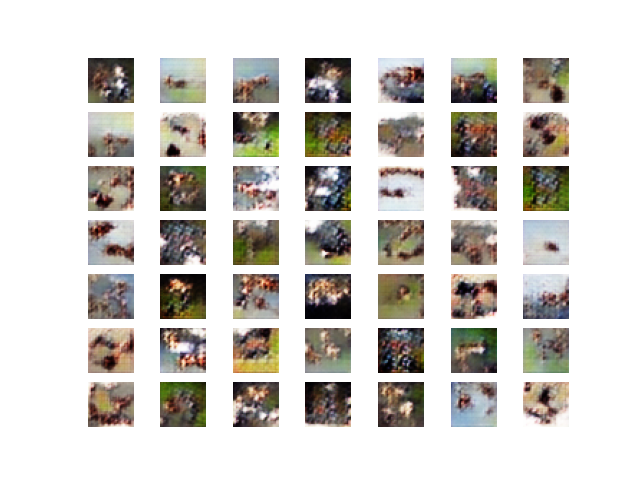
\includegraphics[width=\textwidth]{e20.png}
    \caption{Generated Image on 20 Epochs}
    \label{fig:compute}
\end{figure}
Similarly, the images started to become little more clearer with increase in the number of epochs to 20 but still they lack clarity.

\begin{figure}[H]
    \centering
    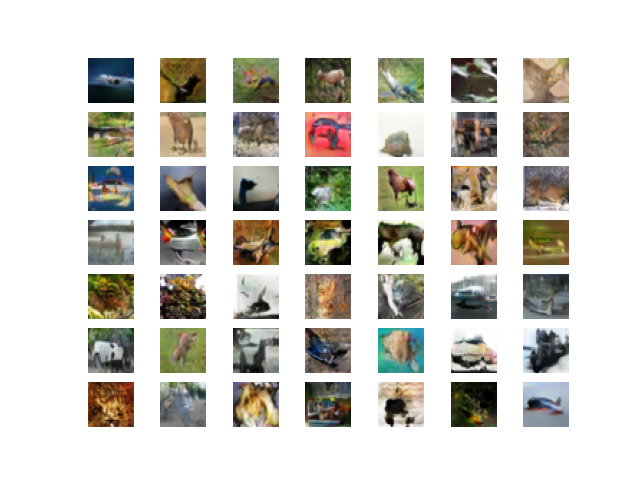
\includegraphics[width=\textwidth]{e200.png}
    \caption{Generated Image on 200 Epochs}
    \label{fig:compute}
\end{figure}
Finally at 200 epochs, we can see plausible photographs with blobs that look like birds, dogs, cats and horses. The objects look familiar to the objects in CIFAR10 dataset, but many of them does not belong to 10 specified classes of CIFAR10 datasets as shown in Figure 9.


\iffalse
\subsection{FMNIST Dataset}
Complete details of hyperparameters used for Fashion-MNIST dataset is stored in Table \ref{tab:CNN-perf} \newline
The experimental result for the FMNIST dataset with various trial run is given as follows:
\vspace{5 mm}
\newline
\textbf{Model Architecture 1}
\subsubsection{Trial Run 1}

Figures \ref{fig:Arch1_Tr1} compares training & testing accuracy and also training & testing loss for Trial Run1. Training accuracy 94.33\% and validation accuracy 88.79\% with no dropout layers and no L2 regularization. In a comparable way, training loss 0.1515 and validation loss 0.50. From trial run 1, inference can be drawn that validation decreases while training increases due to overfitting problem. Therefore, some sort of regularization is needed to alleviate this problem.

\begin{figure}[H]
    \centering
    \subfloat{{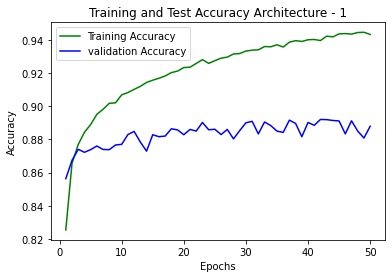
\includegraphics[width=0.465\textwidth]{Arch1_TR1(a).png} }}%
    \qquad
    \subfloat{{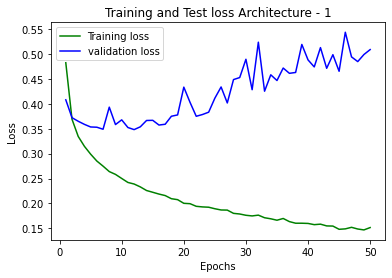
\includegraphics[width=0.465\textwidth]{Arch1_TR1(b).png} }}%
    \caption{Training vs validation accuracy and Loss curve for Arch 1 TR1}%
    \label{fig:Arch1_Tr1}%
\end{figure}

\subsubsection{Trial Run 2}
Figures \ref{fig:Arch1_Tr2} describe the variation in training loss vs testing accuracy and training vs testing loss values respectively when dropout of 0.2 and L2 regularization were added with a learning rate of 0.001. Figure \ref{fig:Arch1_Tr2}
\begin{table}[h]
\centering
\caption{Results for Architecture 1 Trial Run 2}
\begin{tabular}{|l|l|}
\hline
Training Accuracy   & 71.06\% \\ \hline
Validation Accuracy & 71.78\% \\ \hline
Training Loss        & 1.3532    \\ \hline
Validation Loss     & 1.3277    \\ \hline
\end{tabular}
\end{table}

\begin{figure}[H]
    \centering
    \subfloat{{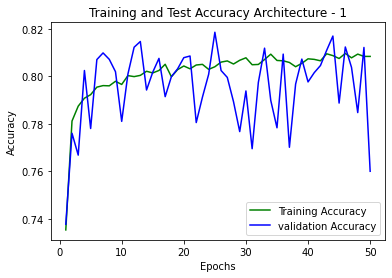
\includegraphics[width=0.465\textwidth]{Arch1_TR2(a).png} }}%
    \qquad
    \subfloat{{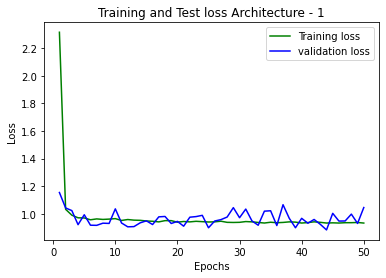
\includegraphics[width=0.465\textwidth]{Arch1_TR2(b).png} }}%
    \caption{Training vs validation accuracy and Loss curve for Arch 1 TR2}%
    \label{fig:Arch1_Tr2}%
\end{figure}

\subsubsection{Trial Run 3}
In trail run 3, dropout was reduced to 0.05 and only L2 regularization was applied with a learning rate of 0.001. From the result, we can see validation accuracy and training accuracy of the model is improved and there is considerable reduction in training loss and validation loss. The results plotted in fig. \ref{fig:Arch1_Tr3} state that an increase in accuracy were observed with a change in hyperparamters as mentioned in the Trial Run 3.

\begin{table}[h]
\centering
\caption{Results for Architecture 1 Trial Run 3}
\begin{tabular}{|l|l|}
\hline
Training Accuracy   & 87.16\% \\ \hline
Validation Accuracy & 85.26\% \\ \hline
Training Loss        & 0.41    \\ \hline
Validation Loss     & 0.48    \\ \hline
\end{tabular}
\end{table}

\begin{figure}[H]
    \centering
    \subfloat{{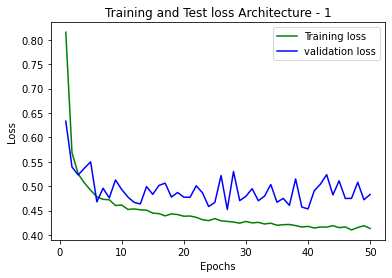
\includegraphics[width=0.465\textwidth]{Arch1_TR3(a).png} }}%
    \qquad
    \subfloat{{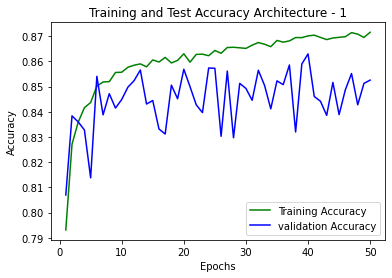
\includegraphics[width=0.465\textwidth]{Arch1_TR3(b).png} }}%
    \caption{Training vs validation accuracy and Loss curve for Arch 1 TR3}%
    \label{fig:Arch1_Tr3}%
\end{figure}


\subsubsection{Trial Run 4}
In fourth trail run we changed the learning rate to 0.0001 which made the optimization much smoother but in 50 epochs, we can only get up to 80.23\% training accuracy and even lower validation accuracy.

\vspace{5 mm}
\newline
\noindent \textbf{Model Architecture 2}

\subsubsection{Trial Run 1}
In model architecture 2 Trial 1, a dense layer was applied with dropout of 20\%, learning rate of 0.0001 and L2 regularization in every dense layer with beta (average momentum) to be 0.95. Results for Training and Testing accuracy could be viewed in Figure \ref{fig:Arch2_Tr1}.

\begin{table}[h]
\centering
\caption{Results for Architecture 2 Trial Run 1}
\begin{tabular}{|l|l|}
\hline
Training Accuracy   & 94.86\% \\ \hline
Validation Accuracy & 89.06\% \\ \hline
Training Loss        & 0.19    \\ \hline
Validation Loss     & 0.4    \\ \hline
\end{tabular}
\end{table}


\begin{figure}[H]
    \centering
    \subfloat{{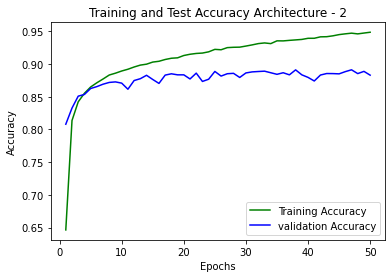
\includegraphics[width=0.47\textwidth]{Arch2_TR1(a).png}}}%
    \qquad
    \subfloat{{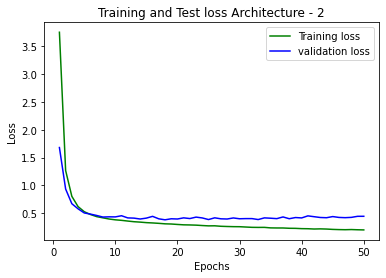
\includegraphics[width=0.47\textwidth]{Arch2_TR1(b).png}}}%
    \caption{Training vs validation accuracy and Loss curve for Arch 2 TR1}%
    \label{fig:Arch2_Tr1}%
\end{figure}

\subsubsection{Trial Run 2}
In the second model architecture, trial 2, a learning rate of 0.0005 was applied with 50\% dropout and L2 regularization on every layer, fig.\ref{fig:Arch2_Tr2} shows the performances with these changes.

\begin{table}[h]
\centering
\caption{Results for Trial Run 2}
\begin{tabular}{|l|l|}
\hline
Training Accuracy   & 91.10\% \\ \hline
Validation Accuracy & 89\% \\ \hline
Training Loss        & 0.3    \\ \hline
Validation Loss     & 0.4    \\ \hline
\end{tabular}
\end{table}

\begin{figure}[H]
    \centering
    \subfloat{{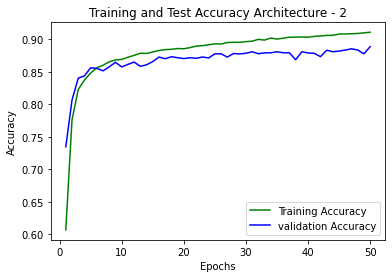
\includegraphics[width=0.47\textwidth]{Arch2_TR2(a).png}}}%
    \qquad
    \subfloat{{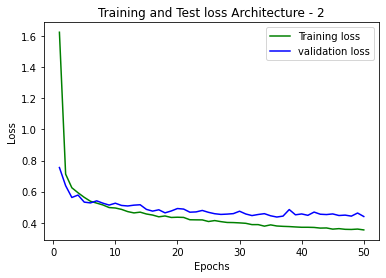
\includegraphics[width=0.47\textwidth]{Arch2_TR2(b).png}}}%
    \caption{Training vs validation accuracy and Loss curve for Arch 2 TR2}%
    \label{fig:Arch2_Tr2}%
\end{figure}

\subsubsection{Trial Run 3 and 4}
In trial run 3 and trial run 4, for model architecture 2, everything remained same as in Trial Run 2 but this time we introduced batch size of 32 and 64, and Dropout of 20\%. respectively.

\begin{table}[h]
\centering
\caption{Results for Trial Run 3 and 4}
\begin{tabular}{|l|l|}
\hline
Training Accuracy   & 90.22\% \\ \hline
Validation Accuracy & 87.82\% \\ \hline
Training Loss        & 0.37    \\ \hline
Validation Loss     & 0.45    \\ \hline
\end{tabular}
\end{table}

\begin{figure}[H]
  \centering
    \subfloat{{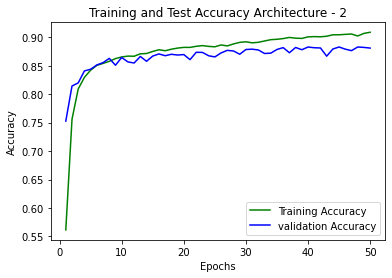
\includegraphics[width=0.47\textwidth]{Arch2_TR3(a).png}}}%
    \qquad
    \subfloat{{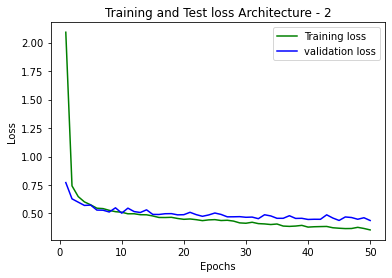
\includegraphics[width=0.47\textwidth]{Arch2_TR3(b).png}}}%
    \caption{Training vs validation accuracy and Loss curve for Arch 3 TR2}%
    \label{fig:Arch2_Tr3}%
\end{figure}
On comparison of Trial Run 3 and 4 where different batch size were used. We do not see a significant difference in both accuracy and loss scores observed in the two cases.

\subsubsection{Confusion Matrix for the Best model}
A confusion matrix is a summary of prediction results on a classification problem. The number of correct and incorrect predictions are summarized with count values and broken down by each class. We plotted the confusion matrix for Fashion-MNIST dataset using scikit-learn library.

\begin{figure}[H]
    \centering
    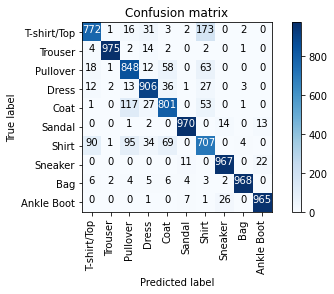
\includegraphics[with=\textwidth]{ConfMatrix.png}
    \caption{Confusion Matrix for best model}
    \label{fig:ConfMatrix}
\end{figure}

\subsection{CIFAR-100 Dataset}
\subsubsection{First Architecture}
In the first architecture, we tried two different learning rates 0.01 and 0.0001. The highest validation accuracy of 0.3 and the lowest validation loss of 2.5 was noted for 0.01 learning rate. fig. \ref{fig:Arch1_CNN(a)} and fig. \ref{fig:Arch1_CNN(b)}

\begin{table}[h]
\centering
\caption{Results for Trial Run 3 and 4}
\begin{tabular}{|l|l|l|}
\hline
Learning rate & 0.01 & 0.0001 \\ \hline
Training Accuracy   & 50\% & 25\% \\ \hline
Validation Accuracy & 30\% & 22\%\\ \hline
Training Loss        & 1.6 & 3.19 \\ \hline
Validation Loss     & 2.5 & 3.11 \\ \hline
\end{tabular}
\end{table}

\begin{figure}[H]
    \centering
    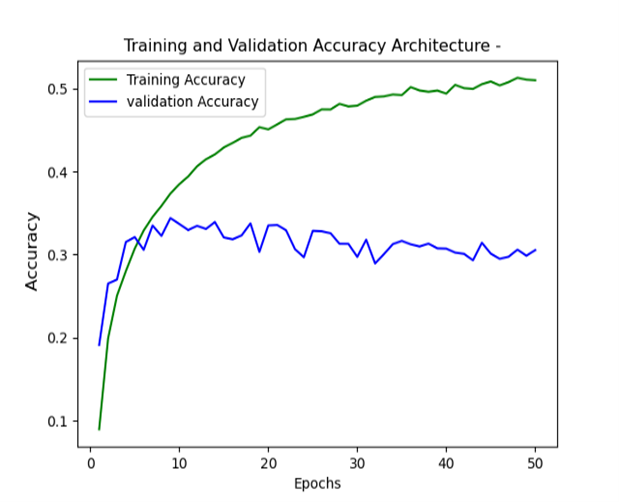
\includegraphics[with=\textwidth]{Conv1_Arch1(b).png}
    \caption{Architecture 1 for CIFAR-100 with LR 0.01}
    \label{fig:Arch1_CNN(b)}
\end{figure}

\begin{figure}[H]
    \centering
    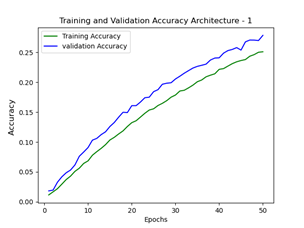
\includegraphics[with=\textwidth]{Conv1_Arch1(a).png}
    \caption{Architecture 1 for CIFAR-100 with LR 0.0001}
    \label{fig:Arch1_CNN(a)}
\end{figure}

\subsubsection{Second Architecture}
In the second module architecture, seven more convolution layers were added including six max pooling layer, L2 linear regularization and dropout of 40\% were added into the model. We obtained the following results: fig. \ref{fig:Arch2_CNN}

\begin{table}[h]
\centering
\caption{Results for Trial Run 3 and 4}
\begin{tabular}{|l|l|}
\hline
Training Accuracy   & 61\% \\ \hline
Validation Accuracy & 39\% \\ \hline
Training Loss        & 1.5    \\ \hline
Validation Loss     & 2.6    \\ \hline
\end{tabular}
\end{table}

\begin{figure}[H]
    \centering
    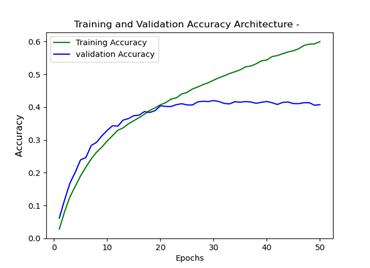
\includegraphics[with=\textwidth]{Conv_arch2.png}
    \caption{Architecture 2 for CIFAR-100}
    \label{fig:Arch2_CNN}
\end{figure}

The above figure shows, training accuracy increases and reach up to 61\% while validation accuracy increases up to 40\% and becomes flatten. This shows even having a smaller learning rate and adding regularization could not solve the problem of overfitting. 


\subsubsection{Third Architecture}
In third architecture, one residual block and one bottleneck layer were added, the training accuracy rose to 90\% in just 15 epochs, but validation accuracy was still lower as shown in the fig. \ref{fig:Arch3_CNN}

\begin{table}[h]
\centering
\caption{Results for Trial Run 3 and 4}
\begin{tabular}{|l|l|}
\hline
Training Accuracy   & 95\% \\ \hline
Validation Accuracy & 42\% \\ \hline
Training Loss        & 0.95 \\ \hline
Validation Loss     & 3.11  \\ \hline
\end{tabular}
\end{table}

\begin{figure}[H]
    \centering
    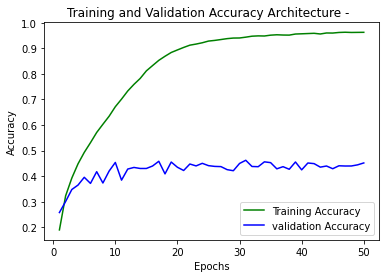
\includegraphics[with=\textwidth]{Conv_Arch3.png}
    \caption{Architecture 3 for CIFAR-100}
    \label{fig:Arch3_CNN}
\end{figure}

 We come to conclusion that the model could perform better with increasing the number of images in the datasets.

\subsubsection{Confusion Matrix for the Best model}
A confusion matrix is a summary of prediction results on a classification problem. The number of correct and incorrect predictions are summarized with count values and broken down by each class. We plotted the confusion matrix for CIFAR-100 dataset using scikit-learn library.

\begin{figure}[H]
    \centering
    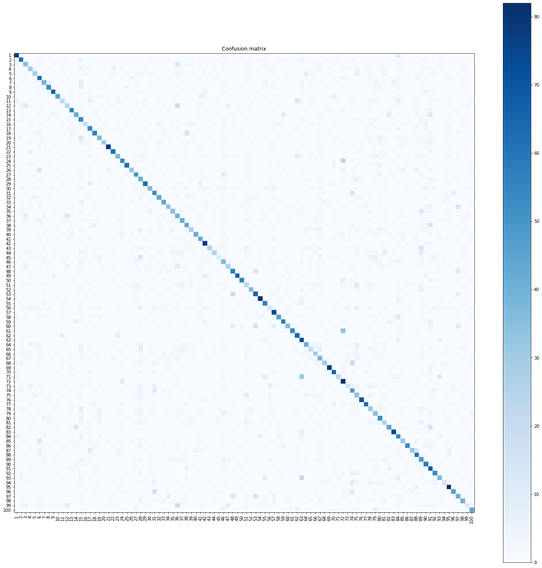
\includegraphics[with=\textwidth]{Conf_Matrix_Cifar100.png}
    \caption{Confusion Matrix for CIFAR-100 best model}
    \label{fig:Conf_matrix_Cifar100}
\end{figure}
\fi

\section{Discussion}
For this homework assignment, we developed a GAN model trained on CIFAR10 dataset. The rounded discriminator loss was around 0.88 with normalized generator loss of 0.924 after 2—epochs, implying that the GAN model was able to reconstruct the images mostly in the correct pixel value range. An important aspect we noticed about the developed model is the fact that there is little overfitting. The fact that there is no overfitting helped us with the decision of increasing the parameter space of both discriminator and generator by increasing the hidden layers. This gave a slightly better performance with a small increase in training time. This assignment helped to understand how to deal with complex architectures. It was tricky to evaluate the performance of the GAN model as we cannot calculate error scores for generated images. To make the training process easier and effective, we calculated FID (Fréchet Inception Distance) scores on real and fake images. We managed to get an FID score varying around 2. To speed up model training we used a GPU (Graphics Processing Units) setup. 


\section{Conclusions}
For the learning problem of this homework assignment, we created a generative model based on GAN (Generative Adversarial Network) architecture using CIFAR10 dataset. To develop this model, hyper-parameters had to be trained from scratch as per the requirements. We measured the model’s performance using the class competition and it got an FID score varying around 2. This homework assignment helped us get a good understanding of the methods to reduce computational complexities involved in dealing with deep architectures. As we did not observe any overfitting in the initial trial runs even with a lesser number of layers in the generator model, we increased the parameter space that enabled the model to give a better performance. Going ahead with this problem, future work could consist of developing a VAE (Variational Auto Encoder) and observing how that architecture compares with the GAN architecture we have already trained. 

\begin{table}[h]
    \caption{Contributions by team member for this assignment.}
    \centering
    \begin{tabular}{|c|c|} \hline
    {\bf Team Member}     &  {\bf Contribution}  \\ \hline
    Shubham Bery     &   Model implementation and result discussion \\
    Shiva Paudel     &   Helping on model implementation and approach description \\
    Puranjit Singh   &   Experimental Results Discussion \\ 
    Kantilata Thapa  &   Helping on model implementation and introducing the problem and datasets \\ \hline
    \end{tabular}
    \label{tab:contribution}
\end{table}

\bibliographystyle{plainurl}
\bibliography{main}

\end{document}